\documentclass[conference]{IEEEtran}
\IEEEoverridecommandlockouts
% The preceding line is only needed to identify funding in the first footnote. If that is unneeded, please comment it out.
\usepackage{cite}
\usepackage{amsmath,amssymb,amsfonts}
\usepackage{algorithmic}
\usepackage{graphicx}
\usepackage{textcomp}
\usepackage{xcolor}
\usepackage{float}
\usepackage{url}
\def\BibTeX{{\rm B\kern-.05em{\sc i\kern-.025em b}\kern-.08em
    T\kern-.1667em\lower.7ex\hbox{E}\kern-.125emX}}
\begin{document}

\title{HOMEWOEK 2}

\author{\IEEEauthorblockN{Runlin Hou}
\IEEEauthorblockA{\textit{ECE, School Of Graduate Studies} \\
\textit{Rutgers University}\\
hourunlinxa@gmail.com}
}

\maketitle

\subsection*{Question 1}
As we known, shellsort would become insertion sort when h reduce to one. 
Meanwhile, the insertion sort will be more efficient when the sequence is 
almost sorted. The shellsort is more efficient because it take a little 
time to sort some shorter sequences divided from the original sequence, 
so that the sequence becomes an almost sorted sequence. By doing so, the 
insertion sort phase can save much more time.

\begin{figure}[H]
    \centerline{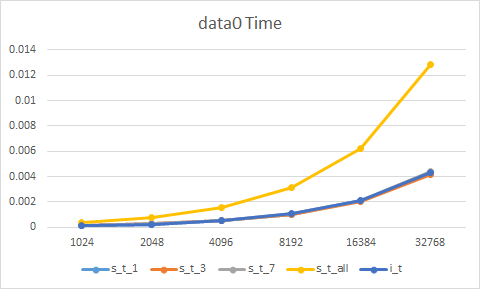
\includegraphics[scale=0.65]{Pic/pic1.png}}
\end{figure}

\begin{figure}[H]
    \centerline{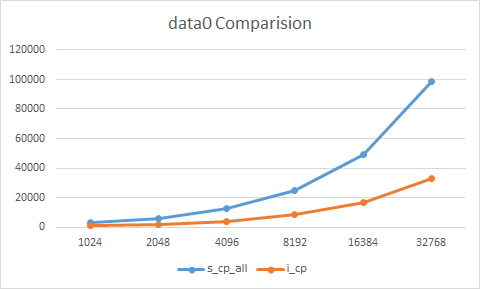
\includegraphics[scale=0.65]{Pic/pic3.png}}
\end{figure}

\begin{figure}[H]
    \centerline{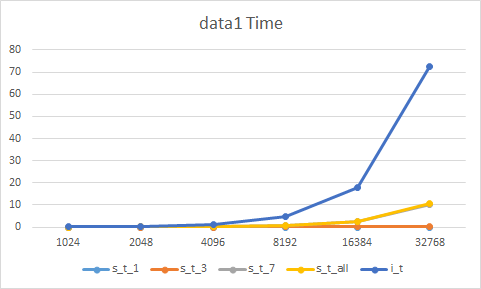
\includegraphics[scale=0.65]{Pic/pic2.png}}
\end{figure}

\begin{figure}[H]
    \centerline{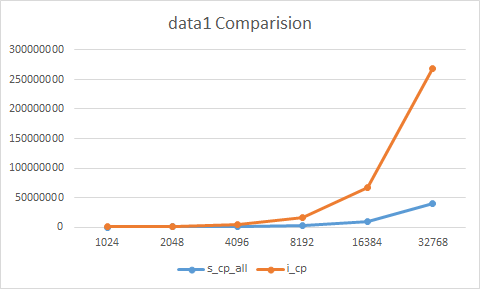
\includegraphics[scale=0.65]{Pic/pic4.png}}
\end{figure}

As we can see in the graph, we deal with a sorted sequence. Time consumption 
and comparision amount of shellsort are both three times of the insertion sort,
since insertion sort just do a traversal but shell do three times.

But as we can see, when we are dealing with a chaotic sequence, insertion sort 
takes much more time and comparision. Because every data is far from where it 
should be, it would takes more comparision to find its position.

\subsection*{Question 2}
The result and time consumption are as follow:

\begin{table}
    \caption{Kendall Tau Distance}
    \begin{center}
        \setlength{\tabcolsep}{9mm}{
        \begin{tabular}{|c|c|}
            \hline
            1024 & 264541\\
            \hline
            2048 & 1027236\\
            \hline
            4096 & 4183804\\
            \hline
            8192 & 16928767\\
            \hline
            16384 & 66641183\\
            \hline
            32768 & 267933908\\
            \hline
        \end{tabular}}
    \end{center}
\end{table}


\begin{figure}[H]
    \centerline{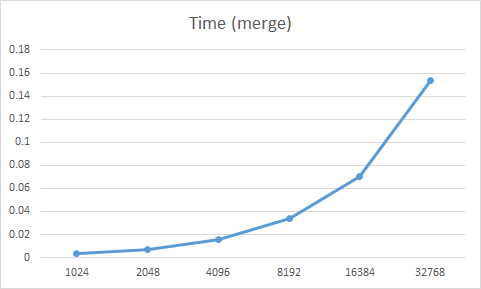
\includegraphics[scale=0.65]{Pic/pic6.png}}
\end{figure}

\begin{figure}[H]
    \centerline{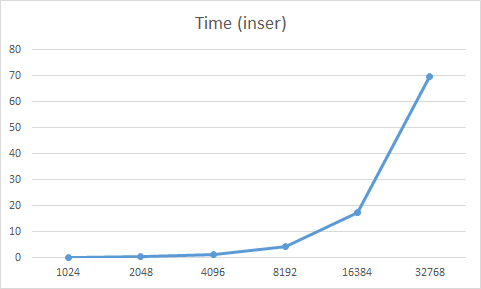
\includegraphics[scale=0.65]{Pic/pic7.png}}
\end{figure}

My basic logic of deciding KTD is to set one sequence as reference sequence, which
means we will take whatever the fisrt value in the reference sequence is the smallest
and whatever the last value in the reference sequence is the largest value. Then we 
will resort the other sequence based on the index of the reference sequence. Then we 
find the inverse pairs in the 2nd sequence, we find the KTD.

The way to decide the amount of inserve pairs would is to find the exchange time of 
a stable sort algorithm. Cause every exchange means the latter value is smaller than
the former value, which is a pair of inverse values.

In my implementatoin, I use both merge sort and insertion sort to find KTD. As expected,
the time consumption refers to $(O(NlogN))$ and $O(N^2)$.

\subsection*{Question 3}
Comparision and array access are the two operations should be consider in merge sort. 
For the comparisions, every time we finish a merge to the whole array takes $N$ comparisions.
And we will take $logN$ whole merge, since every time will take half of the array to 
merge together. 

And for array access operation, we can decide from the amount of merge happens. Every merge
is going to take a comparision, which means two read of arrays. And after deciding the smaller
value, we will write it to the auxiliary array, which means one read from the original array 
and one write to the auxiliary array. Then we will write the value from auxiliary array back to
original array, which mean one read from auxiliary array and one write to the original array.
So we total have 6 array access in each merge, 2 writes and 4 reads. For whole process we will
have $6NlogN$ array access.


\begin{figure}[H]
    \centerline{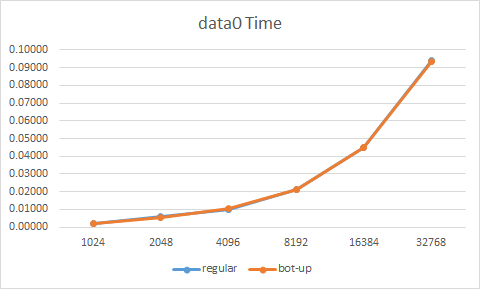
\includegraphics[scale=0.65]{Pic/pic8.png}}
\end{figure}

\begin{figure}[H]
    \centerline{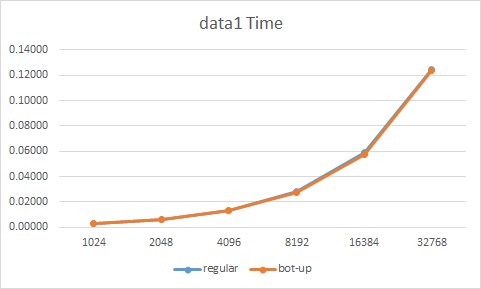
\includegraphics[scale=0.65]{Pic/pic9.png}}
\end{figure}

From the time consumption we can see that the two algorithm as expected have a pretty 
similar time consumption.

\subsection*{Question 4}
For this problem, I assume we know that the sequence we are going to deal with has 
1024 repeats of 1, 2048 repeats of 11, 4096 repeats of 111 and 1024 repeats of 1111.
So I set four pointers in a auxiliary array points to the positions where the 4 entities 
are supposed to start. So whin one traversal, I can set the entity into where it 
should be by moving the pointers. Then we write back this auxiliary array to sort it.
The process rakes $N$ comparisions and $2N$ writes. Which I think should be the smallest
time consumption.

\subsection*{Question 5}


\end{document}